\chapter{Conceptos Previos}

Este cap\'itulo introduce el marco te\'orico del presente trabajo a trav\'es de 
la definici\'on de los siguientes conceptos: espacios m\'etricos (ejemplo: diccionario de 
palabras), medidas de distancia; se incluyen algunas de las medidas m\'as comunes utilizadas 
dentro de la tem\'atica a tratar, e introduciremos un modelo formal para las b\'usquedas por 
similitud.

\section{Espacios M\'etricos}

En este trabajo se aborda el tema de b\'usqueda no convencional, es decir, dentro de un universo 
de datos, nos interesa encontrar aquellos objetos que son "similares" a un objeto dado. El modelo 
formal que abarca este tipo de b\'usquedas se denomina Espacio M\'etrico.

Espacio M\'etrico:
Sea $X$ un universo de objetos v\'alidos y sea $U \subseteq X$ un subconjunto finito de tama\~no n 
sobre el que se realizar\'an b\'usquedas. Llamaremos $U$ a las base de datos, diccionario o 
simplemente conjunto de elementos.
Definimos una funci\'on $d:(X \times X) \rightarrow \Re$ que denotar\'a una medida de distancia 
entre objetos de $X$, esto significa que a menor distancia m\'as cercanos o similares son los 
objetos. Esta funci\'on $d$ cumple con las propiedades caracter\'isticas de una funci\'on de 
distancia:


\begin{enumerate}
\item [(a)] $\forall x,y \in X d(x,y) \geq 0$ (Positividad)
\item [(b)] $\forall x,y \in X d(x,y) = d(y,x)$ (Simetr\'ia)
\item [(c)] $\forall x \in X d(x,x) = 0 $ (Reflexividad)
\end{enumerate}
en la mayor\'ia de los casos:
\begin{enumerate}
\item [(d)]  $\forall x,y \in X x \neq y \Rightarrow > 0$ (Positividad estricta)
\end{enumerate}


Estas propiedades s\'olo aseguran una definici\'on consistente de la funci\'on, pero no pueden 
usarse para evitar comparaciones durante una b\'usqueda por similitud. Para que la funci\'on d sea 
realmente una m\'etrica debe satisfacer la siguiente propiedad:

\begin{enumerate}
\item  [(e)] $\forall x,y,z \in X d(x,y) \leq d(x,z) + d(y,z)$ (Desigualdad triangular)
\end{enumerate}

El par $X,d$ es llamado espacio m\'etrico. Si la funci\'on $d$ no satisface la propiedad de 
positividad estricta (d), entonces diremos que el espacio es pseudo m\'etrico. Estos casos pueden 
ser f\'acilmente resueltos; basta con adaptar las t\'ecnicas de espacios m\'etricos de manera tal 
que todos los objetos a distancia cero se identifiquen como un \'unico objeto. Esto funciona dado 
que $d(x,x) = 0 \Rightarrow \forall z, d(x,z) = d(y,z)$ (puede demostrarse utilizando la 
desigualdad triangular).

En algunos casos podemos tener cuasi m\'etricas donde no se cumpla la propiedad de simetr\'ia (b). 
En estos casos podemos definir a partir de la funci\'on $d$ una nueva funci\'on $d'$, que s\'i sea 
m\'etrica $d'(x,y) = d(x,y) + d(y,x)$.

Finalmente podemos llegar a relajar la desigualdad triangular (e) permitiendo $d(x,y)  \leq \alpha 
d(x,z) +  \beta d(z,y) + \gamma$. En estos casos podemos seguir usando los mismos algoritmos de 
espacio m\'etrico, previo escalamiento.


\section{B\'usquedas por similitud}
B\'asicamente existen tres tipos de b\'usquedas de inter\'es en
espacios m\'etricos \cite{oursurvey}:

\begin{description}
   \item {\textbf{B\'usqueda por rango $(q,r)_{d}$:}}
          consiste en recuperar todos los elementos  de $\mathcal{U}$
          que est\'an a distancia $r$ de un elemento $q$ dado (que llamaremos
          query).  En s\'imbolos:
           \vspace{-3mm}
          \[(q,r)_{d}=\{u \in \mathcal{U}:  d(q,u) \leq r\}\]
          
          Son probablemente las m\'as comunes dentro de los espacios
           m\'etricos.  Los objetos pertenecientes a la respuesta pueden 
           ordenarse en base a su distancia de $q$, si es necesario.
            N\'otese que el objeto $q$ no necesita existir en la base de datos $U$,
            basta con que sea un elemento del universo $X$, 

   \item{\textbf{ B\'usqueda del vecino m\'as cercano $NN(q)$:}}
         Cuando se quiere realizar b\'usquedas por similitud sobre objetos 
         utilizando b\'usquedas por rango, se debe especificar la distancia 
         m\'axima para que los objetos sean inclu\'idos en la respuesta. Existen 
         casos donde puede ser dif\'icil especificar el radio sin conocimiento
          sobre los datos y la funci\'on de distancia. 
          Se no presenta entonces la situaci\'on en donde, si especificamos 
          un radio de b\'usqueda muy peque\~no no obtendremos ning\'un resultado, 
          y deberemos repetir la b\'usqueda con un radio mayor. 
          Por otro lado, si especificamos un radio de b\'usqueda 
          muy grande, corremos el riesgo de que el costo computacional de calcular 
          la distancia sea muy alto y de que el conjunto de resultados contenga 
          objetos no significativos. 
          Una alternativa para solucionar este tipo de problemas en la b\'usqueda por
           similitud es realizar una b\'usqueda de el (o los)  vecino(s) m\'a(s) cercano(s)
           a $q$. Esta b\'usqueda se define de la siguiente manera:
          \vspace{-3mm}
          \[ NN(q)=\{u \in \mathcal{U} : \forall v \in \mathcal{U},
          \ d(q,u) \leq d(q,v)\}\]
          

   \item {\textbf{ B\'usqueda de los k-vecinos m\'as cercanos $NN_{k}(q)$:}}
         El concepto de vecino m\'as cercano puede generalizarse al caso 
         de b\'usqueda de los $k$ vecinos m\'as cercanos. Espec\'ificamente
          $kNN(q)$ retorna los $k$ vecinos m\'as cercanos del objeto $q$, 
          Esto significa encontrar un conjunto
          $A \subseteq \mathcal{U} $ tal que:
          \vspace{-3mm}
         \[|A| =k \ \wedge \forall u \in A,\  v \in ( \mathcal{U} - A) :
          \ d(q,u) \leq d(q,v)\]
          
          Cuando existen varios objetos a la misma distancia del $k$-\'esimo 
          vecino m\'as cercano, la elecci\'on de uno se realiza arbitrariamente.
           
\end{description}

El tiempo total de resoluci\'on de una b\'usqueda puede ser calculado de la
siguiente manera:

\centerline{
    \em T= \#evaluaciones  de $d \times $ complejidad(d) +  tiempo extra de
    CPU + tiempo de  I/O
}

En muchas aplicaciones  la evaluaci\'on de la funci\'on $d$ es tan costosa
que las dem\'as componentes de la f\'ormula anterior pueden ser despreciadas.
\'este es el modelo de costos  que usaremos en este trabajo.

Claramente una b\'usqueda por similitud puede resolverse de forma
ineficiente en tiempo  $O(n)$ examinando exhaustivamente la base de datos $\mathcal{U}$.
Para evitar esto, se preprocesa $\mathcal{U}$ usando alg\'un {\em algoritmo de
indexaci\'on} que construye  un 
\'indice, dise\~nado  para ahorrar c\'omputos en el momento de resolver una b\'usqueda.
El proceso de  construcci\'on del \'indice puede ser costoso, pero este costo
se ver\'a justificado por el gran n\'umero de consultas que posteriormente se
realizar\'an en la base de datos.

Hay dos casos principales a considerar: cuando el \'indice y los datos pueden ser
mantenidos en memoria principal, y cuando es necesario utilizar memoria secundaria
para almacenar los datos y/o el \'indice. Para los algoritmos de indexaci\'on
en memoria principal, el objetivo principal es reducir el n\'umero de c\'alculos de distancia
(se adec\'ua al modelo que mencion\'aramos anteriormente).
  Para los algoritmos en memoria secundaria, adem\'as
de realizar pocos c\'alculos de distancia, se requiere que tambi\'en realicen
pocos accesos a disco. 


\section{Ejemplos de Espacios M\'etricos}

Veremos a continuaci\'on algunos ejemplos de espacios m\'etricos.

\noindent \textit{\textbf{Diccionario de Palabras}}

En este caso, los objetos del espacio m\'etrico son cadenas de caracteres de un determinado 
lenguaje. Para medir la distancia entre cadenas, una funci\'on posible es la conocida como 
distancia de edici\'on o distancia de Levenshtein, que mide el m\'inimo n\'umero de operaciones
 de inserci\'on, eliminaci\'on y reemplazo de caracteres necesarias  para transformar una palabra $x$ 
 en una palabra $y$. 


Claramente, esta es un funci\'on de distancia discreta y tiene una variedad de aplicaciones
en recuperaci\'on de texto procesamiento de se\~nales y biolog\'i­a computacional.
Como veremos mas adelante, en este trabajo hemos utilizado un espacio m\'etrico 
similar al diccionario de palabras, ya que nuestro 
universo de objetos se compone de t\'itulos de productos en venta publicados en 
un sitio de e-commerce.

\noindent \textit{\textbf{Espacios vectoriales}}

Los espacios vectoriales $k$-dimensionales son un caso especial de espacios m\'etricos, donde los
objetos son vectores de $k$ componentes. Hay varias funciones de distancia para espacios 
vectoriales, pero las m\'as usadas son las pertenecientes a la familia $L_p$ o familia de 
distancias de Minkowsky (veremos su definici\'on en la pr\'oxima secci\'on)



\begin{figure}[tb]
\centerline{%
  \begin{tabular}{|c|c|} \hline
   &  \\
     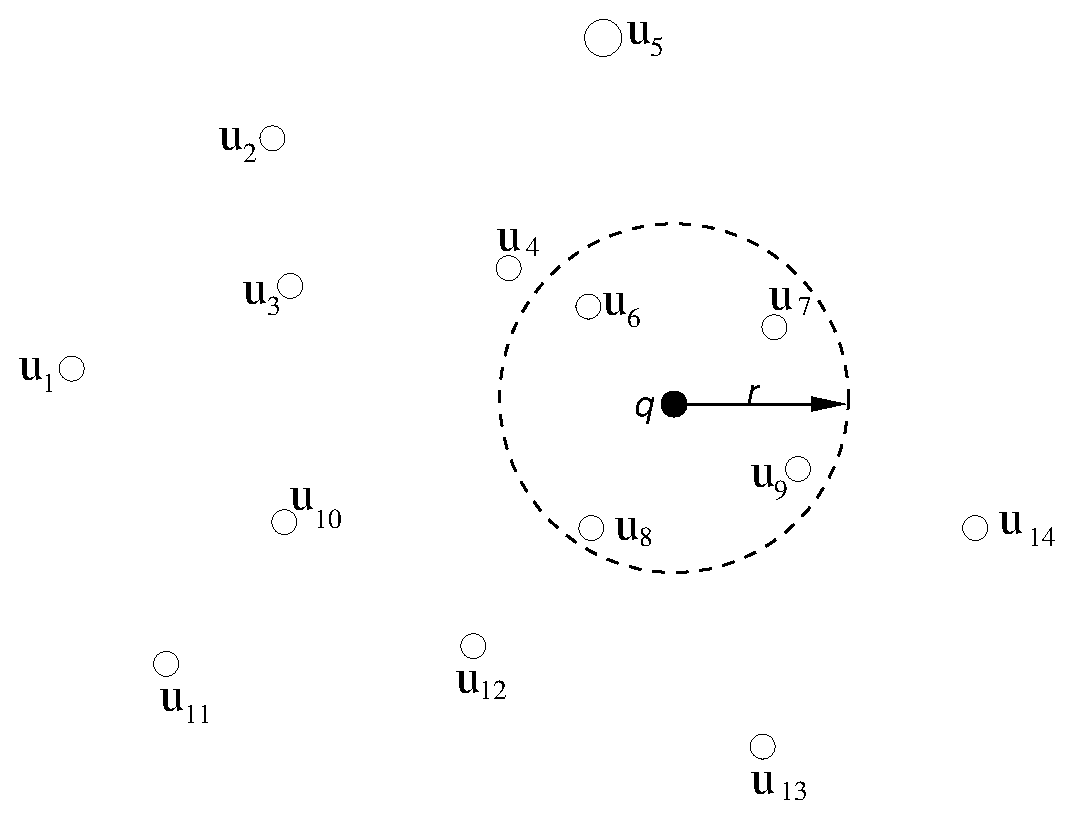
\psfig{file=imagenes/query-rangoL2.eps,width=70mm} &
     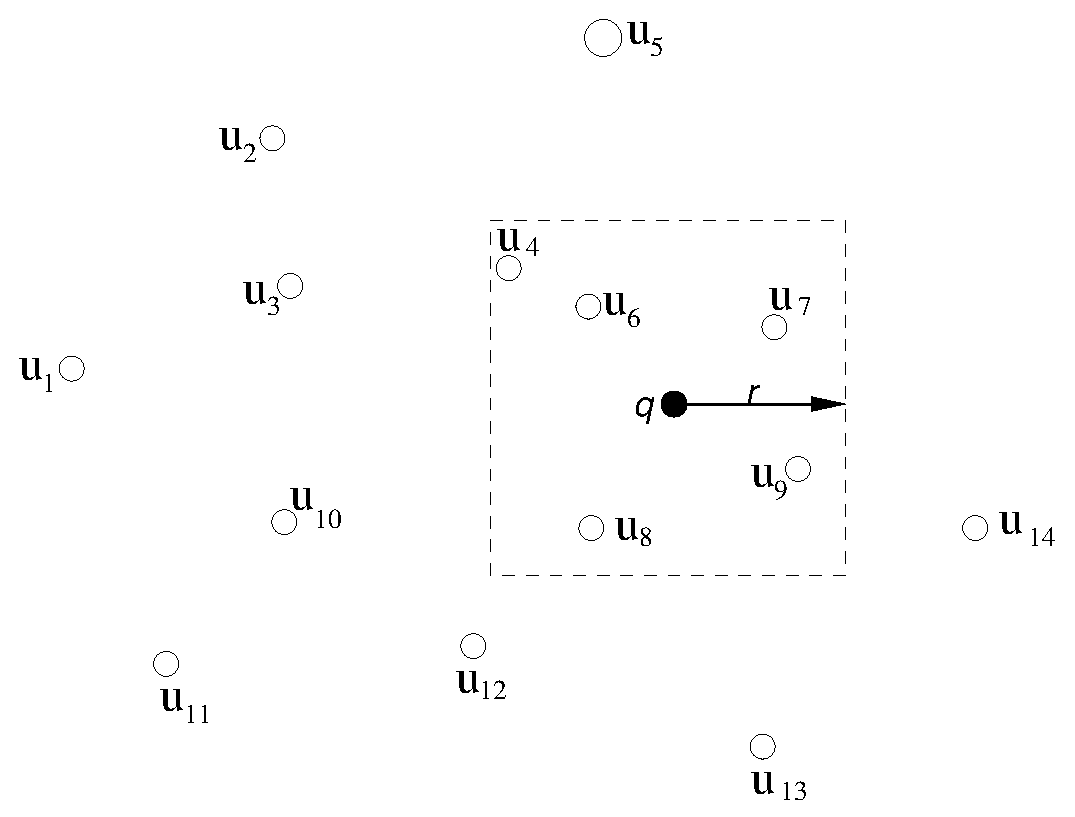
\psfig{file=imagenes/query-rangoLI.eps,width=70mm} \\ \hline
  \end{tabular}}
  \caption [Ejemplos de b\'usquedas por rango $(q,r)_d$ en   $\mathbb{R}^2$]
     {\textsl{\footnotesize { Ejemplos de b\'usquedas por
      rango $(q,r)_d$, con $d=L_2$ (izquierda) y $d=L_\infty$ (derecha). }}}
\label{query-rango}
\end{figure}


La Figura \ref{query-rango} ejemplifica b\'usquedas por rango $(q,r)_d$ sobre un 
conjunto de puntos en $\Re^2$, usando como funci\'on de distancia $L_2$ (izquierda) 
y $L_{\infty}$ (derecha), dos casos particulares de la distancia $L_p$.
Las l\'ineas punteadas representan aquellos puntos que est\'an ex\'actamente a distancia
$r$ de $q$, por lo tanto todos aquellos elementos que caen dentro de estas l\'ineas 
forman parte del resultado de la b\'usqueda. La distancia $L_2$, m\'as conocida como
\textit{Distancia Euclidiana}, se corresponde con nuestra noci\'on de distancia espacial.
 Las b\'usquedas con distancia $L_{\infty}$ se corresponde con la b\'usqueda por rango
cl\'asica, donde el rango es un hiper-rect\'angulo $k$ dimensional.

En el \'ambito de espacios vectoriales existen soluciones eficientes para b\'usquedas por
similitud, como por ejemplo: $KD-tree$, $R-tree$, $Quad tree$ y $X-tree$ entre otras. Estas
t\'ecnicas usan informaci\'on sobre coordenadas para clasificar y agrupar puntos en el espacio. 
Desafortunadamente, las t\'ecnicas existentes son afectadas por la dimensi\'on del espacio 
vectorial. Por lo tanto, la complejidad de b\'usqueda por rango depende exponencialmente de la 
dimensi\'on del espacio.
 
Los espacios vectoriales pueden presentar grandes diferencias entre su dimensi\'on 
representacional y su dimensi\'on intr\'inseca (es decir la dimensi\'on real en la que se pueden 
embeber los puntos manteniendo la distancia entre ellos). Por ejemplo, un plano embebido en un 
espacio de dimensi\'on 50, tiene una dimensi\'on representacional de 50 y una dimensi\'on 
intr\'inseca de 2.

Por esta raz\'on, muchas veces se recurre a espacios m\'etricos generales, aun sabiendo que el 
problema de b\'usqueda es m\'as dif\'icil. No se debe descartar que tambi\'en es posible tratar un 
espacio vectorial como un espacio m\'etrico general usando solo la distancia entre los puntos. Una 
ventaja inmediata de esto es que toma peso la dimensi\'on intr\'inseca del espacio, 
independientemente de cualquier dimensi\'on representacional.

\section{Funciones de Distancia}

Cuando hablamos de funciones de distancia, podemos dividirlas en dos grupos, de acuerdo
 al tipo de valor que retornan:

\begin{itemize}
\item \textbf{Discretas}: son  aquellas que retornan un valor discreto como valor de 
distancia, como por ejemplo la distancia de edici\'on.

\item \textbf{Continuas}: son las que retornan un n\'umero real como distancia entre
objetos, como por ejemplo la distancia $L_2$ o distancia Euclidiana.

\end{itemize}


Describimos a continuaci\'on algunos ejemplos de funciones de distancia para
espacios m\'etricos. 

\noindent \textbf{\textit{Distancia de Minkowski}} 

Como ya lo mencionamos, estas funciones forman realmente una familia de 
funciones denominadas m\'etricas $L_p$, ya que los 
casos individuales dependen del par\'ametro num\'erico $p$. Estas funciones se definen sobre 
vectores $K$-dimensionales de n\'umeros reales de la siguiente manera:

\[
L_p[(x_1,\ldots,x_K),(y_1,\ldots,y_K)] = \sqrt[p]{ \sum_{i=1}^k|x_i - y_i|^p}
\]

La m\'etrica $L_1$ es conocida como la distancia de Manhattan y la m\'etrica
 $L_2$ denota la distancia Euclidiana.
Para el caso de $p=\infty$, se toma el l\'imite de la f\'ormula anterior para $p$ tendiendo $
\infty$. Se obtiene como resultado, que la distancia entre dos puntos del espacio vectorial es la 
m\'axima diferencia entre sus coordenadas:

\[
L_{\infty}((x_1,...,x_k), (y_1,...,y_k)) = max_{1 \leq i \leq k} |x_i - y_i |
\]

 
 La funci\'on $L_{\infty}$ se conoce con el nombre de  distancia m\'axima, infinita o distancia de tablero de ajedrez.

Estas funciones son utilizadas en varios casos donde los vectores num\'ericos 
tienen condenadas independientes, por ejemplo, en mediciones de experimentos cient\'ificos, observaciones ambientales, o el estudio de diferentes aspectos de procesos de negocios.

\noindent \textbf{\textit{Distancia de  forma cuadr\'atica}}

En muchas aplicaciones que utilizan vectores de datos, los valores de las distintas 
dimensiones no son totalmente independientes. En estos casos las distancias de Minskowski
no son aplicables ya que no tienen en cuenta la existencia de esta relaci\'on.

La distancia de forma cuadr\'atica  es utilizada en \'ambitos en los que existe
 una correlaci\'on entre  las dimensiones que componen el vector, ya que tiene 
 el poder de modelar este tipo de  dependencias. La medida de distancia entre 
 dos vectores $\bar{x}$ e $\bar{y}$  de $k$ dimensiones est\'a basada en una matriz
 positiva de pesos   $M_{k \times k}$ donde 
$m_{i,j}$  denotan cu\'an fuerte es la conexi\'on entre los componentes $i$ y $j$ de los vectores 
$\bar{x}$ e $\bar{y}$, respectivamente. Generalmente estos pesos son normalizados de manera que 
$0\leq m_{i,j} \leq 1$ donde las diagonales $m_{i,	i} = 1$.
La distancia de forma  cuadr\'atica generalizada $d_M$ se define como:

\[
d_M(\bar{x},\bar{y}) = \sqrt{(\bar{x} - \bar{y})^T \cdot M \cdot (\bar{x} - \bar{y})}
\]

\noindent donde el super\'indice $T$ denota la transposici\'on de vectores.

El c\'alculo de \'esta distancia puede ser muy caro en t\'erminos computacionales, dependiendo de la dimensionalidad de los vectores.
Notar que $M$ es la matr\'iz identidad, esta distancia se transforma en la distancia
euclidiana.

\noindent \textbf{\textit{Distancia de Edici\'on}}

La cercan\'ia entre secuencias de s\'imbolos (cadenas) puede medirse de manera efectiva a trav\'es 
de la distancia de Edici\'on, tambi\'en conocida como distancia de Levenshtein. La distancia entre 
dos cadenas $x=x_1...x_n$ e $y=y_1...y_n$ est\'a definida como el n\'umero m\'inimo de operaciones 
at\'omicas de edici\'on (inserci\'on, eliminaci\'on y reemplazo) necesarias para transformar la 
cadena $x$ en la cadena $y$. En t\'erminos formales, las operaciones de edici\'on se definen como 
sigue:

\begin{itemize}
\item \textbf{insert:} inserci\'on del caracter $c$ en la posici\'on $i$
de la cadena $x$, en s\'imbolos: 
\[ins(x,i,c)=x_1 x_2 \ldots x_i\ c\ x_{i+1} \ldots x_n\]
 
\item  \textbf{delete}: eliminaci\'on del caracter $c$ en la posici\'on 
$i$ de la cadena $x$, en s\'imbolos:
  \[ del(x,i)=x_1 x_2 \ldots x_{i-1} x_{i+1} \ldots x_n\]
  
  
\item \textbf{replace}: sustituci\'on de un caracter $c$ de la cadena $x$ en 
la posici\'on $i$ por un nuevo caracter $c'$, en s\'imbolos:
\[repl(x,i,c)=x_1 x_2 \ldots x_{i-1}\ c' \ x_{i+1} \ldots x_n\]
\end{itemize}


La funci\'on de distancia de edici\'on generalizada asigna pesos (n\'umeros reales positivos) a 
cada operaci\'on at\'omica, por esto, la distancia entre las cadenas $x$ e $y$ es el m\'inimo 
valor de la suma de los pesos de las operaciones at\'omicas necesarias para transformar $x$ en $y
$. Si los pesos asignados a cada operaci\'on difieren, la distancia de edici\'on no es sim\'etrica 
(violando la propiedad (b) del punto 2.1) y por lo tanto, no es una funci\'on m\'etrica.


A los fines del presente trabajo, a todas las operaciones se le asigna un peso equivalente de uno.

\noindent \textbf{\textit{Distancia de Edici\'on de \'arbol}}

Esta distancia es una bien conocida medida de proximidad entre \'arboles, en la cual se define la 
distancia entre dos estructuras de \'arboles como el costo m\'inimo necesario para convertir el 
\'arbol fuente en el \'arbol destino utilizando un conjunto predefinido de operaciones de edici
\'on sobre \'arboles, tales como la inserci\'on y la eliminaci\'on de un nodo. El costo individual 
de estas operaciones de edici\'on puede ser constante para todo el \'arbol, o puede variar de 
acuerdo al nivel en el cual se lleva a cabo la operaci\'on. La raz\'on de esta variaci\'on es que 
el costo de la inserci\'on de un nodo cercano al nivel de la ra\'iz puede ser m\'as significativo 
que el costo de agregar un nodo hoja. Por supuesto, esto depende del dominio de aplicaci\'on.

Dado que los documentos XML generalmente se modelan como \'arboles etiquetados, esta distancia 
puede utilizarse tambi\'en para medir las diferencias estructurales entre dos documentos XML.

\noindent \textbf{\textit{Coeficiente de Jaccard}}

Si quisi\'eramos medir la distancia en un tipo diferente de datos, como lo son los conjuntos, 
podemos utilizar el denominado coeficiente de Jaccard. Asumiendo dos conjuntos $A$ y $B$, el 
coeficiente de Jaccard se define como:
\[
d(A,B) = 1 - \frac{|A \cap B|}{|A\cup B|}
\]

Esta funci\'on se basa simplemente en la raz\'on entre las cardinalidades de la intersecci\'on y 
la uni\'on de los conjuntos comparados. Como un ejemplo de una aplicaci\'on que trabaja con 
conjuntos, supongamos que tenemos un registro con usuarios y direcciones de sitios web que 
visit\'o cada uno. Para evaluar la similitud en el comportamiento de cada usuario, podemos 
utilizar el coeficiente de Jaccard.


\section{Algoritmos de Indexaci\'on}

Los algoritmos de indexaci\'on sirven para organizar la informaci\'on o universo de datos en
 estructuras de datos o \'indices. Este pre proceso de la base de datos tiene como objetivo
  reducir el n\'umero de c\'alculos al momento de resolver una b\'usqueda. Un dise\~no eficiente 
  de los \textit{algoritmos de indexaci\'on}, junto con la desigualdad triangular, permite 
  descartar   elementos evitando comparar la query con cada uno de los elementos de la base o 
  universo de datos. As\'i, dada una query, primero se recorre el \'indice para determinar un 
  subconjunto de elementos candidatos a ser parte de la respuesta y luego se examinan esos 
  conjuntos en forma exhaustiva para obtener la respuesta definitiva.

\subsection{Un Modelo Unificado}

Todos los algoritmos de indexaci\'on particionan la base de datos $U$ en subconjuntos $U_I$. El \'indice permite identificar una lista de $U_i$ que potencialmente contiene elementos significativos para la consulta. Por consiguiente, la b\'usqueda se reduce a:

\begin{itemize}
\item Recorrer el \'indice para obtener los  candidatos. El costo de este proceso se denomina \textit{complejidad interna}

\item Examinar exhaustivamente estos candidatos  a fin de encontrar los elementos que realmente forman el resultado de la b\'usqueda. El costo de este proceso se denomina \textit{complejidad externa}. 

\end{itemize}

\begin{figure}[tb]
\centerline{%
  \begin{tabular}{c c c}
  \\
     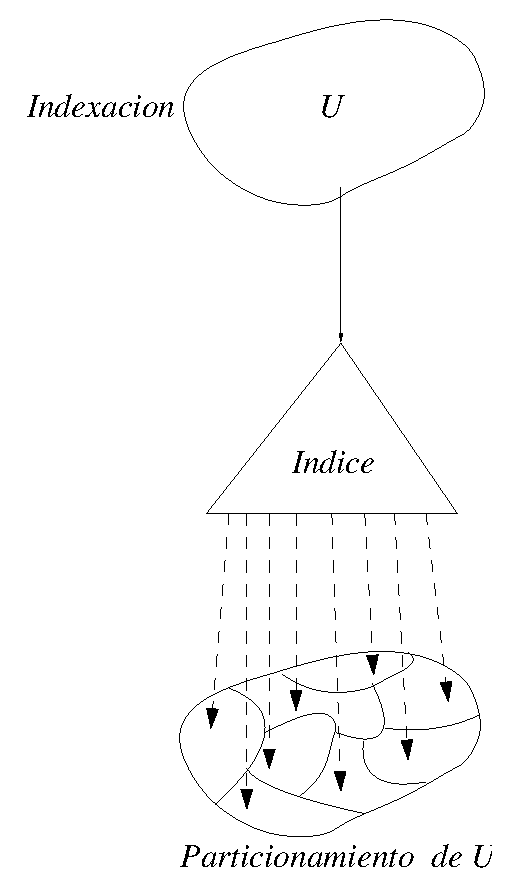
\psfig{file=imagenes/ejem-indice.eps,width=35mm} & \hspace{3cm}
     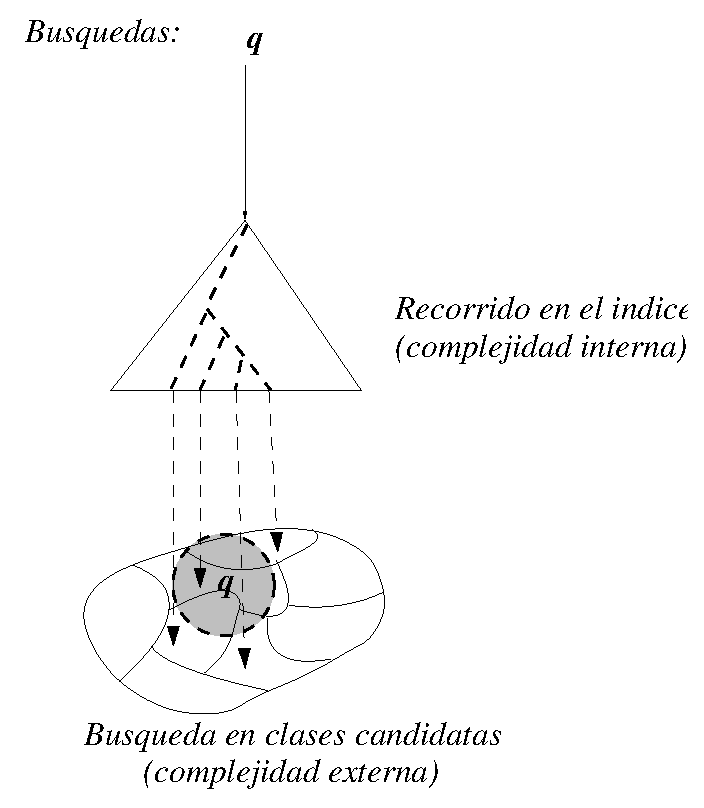
\psfig{file=imagenes/ejem-indice-bsq.eps,width=55mm}
  \end{tabular}}
  \caption[Modelo general de algoritmos de indizaci\'on]
  {\textsl{\footnotesize{ Modelo general de algoritmos de indexaci\'on para Espacios M\'etricos. }}}
\label{modelo-gral-indices}
\end{figure}

La Figura \ref{modelo-gral-indices} ejemplifica este modelo general de
indexaci\'on. La figura de la izquierda muestra la divisi\'on en clases de equivalencia
del espacio m\'etrico. La figura de la derecha muestra las clases de equivalencia que 
potencialmente contienen elementos relevantes para una b\'usqueda $q(r,d)$.

Para comprender totalmente el proceso de indexaci\'on se necesita entender 
adecuadamente los conceptos de relaci\'on de equivalencia y partici\'on de conjuntos.
 Aqu\'i, la relevancia de dichos conceptos se debe a la posibilidad de particionar 
 un espacio m\'etrico en clases de equivalencias y obtener as\'i un nuevo espacio
  m\'etrico derivado del conjunto cociente.

Toda partici\'on $\pi(X) = \{\pi_1, \pi_2,...., \pi_n\}$ de un conjunto $X$ induce una relaci\'on de equivalencia (que denotamos con \~). Inversamente toda relaci\'on de equivalencia induce una partici\'on:

 \[
\forall x,y  \in X: x ~ y  \Leftrightarrow x \mbox{est\'a en la misma parte que} y
\]


Las clases de equivalencia $[x]$ de esta relaci\'on se corresponden con las partes $\pi_i$ de la partici\'on $\pi$, es decir,

\[
\pi(X) = X/~
\]


Por consiguiente, los algoritmos de indexaci\'on existentes definen una relaci\'on de equivalencia 
sobre el espacio m\'etrico $X$. Las clases de equivalencia de $X$ en el conjunto cociente $\pi(X)$ 
pueden considerarse como elementos de un nuevo espacio m\'etrico, bajo alguna funci\'on de 
distancia $D: \pi(X)  \times \pi(X) \rightarrow  \Re^+$.

Ahora definimos la funci\'on $D_0$ que ser\'a de utilidad para encontrar la funci\'on $D$

\[
D_0: 	\pi(X) \time \pi(X)  \rightarrow \Re^+
D_0([x],[y]): \min_{x \in [x], y \in [y]}\{d(x,y)\}
\]
			
$D_0$ representa la menor distancia entre un elemento de la clase $[x]$ y un elemento de la clase 
$[y]$. Esta distancia es el m\'aximo valor posible que mantiene el mapeo contractivo, es decir que 
$\forall x,y \in X : D_0([x],[y]) \leq d(x,y)$.
					
$D_0$ no puede ser utilizada con la finalidad de indexaci\'on porque no satisface la desigualdad 
triangular pero nos aproxima a una soluci\'on dado que sabemos que cualquier funci\'on de 
distancia $D$, que adem\'as cumple con las propiedades para ser una m\'etrica, es una cota 
inferior de $D_0$ (manteniendo as\'i el mapeo contractivo) que nos sirve para definir un nuevo 
espacio m\'etrico. En otras palabras, esta nueva funci\'on $D$ debe cumplir que $\forall [x],[y] 
en \pi(X),  D([x],[y]) \leq D_0([x],[y])$.

Luego, podemos convertir un problema de b\'usqueda en otro, que esperamos sea m\'as sencillo. 
Para una b\'usqueda $(q, r)_d$ primero, buscamos espacio $\pi(X, D)$ obteniendo como resultado $([q], r)_D = \{u \in  U/ D([u],[q]) \leq r\}$. Como $D_0$  es contractiva, podemos asegurar que $(q, r)_d \subseteq ([q], r)_D$.  Luego realizamos una b\'usqueda exhaustiva en $([q], r)_D$ a fin de determinar los elementos que forman parte de la respuesta a la consulta $(q, r)_d$.
				
Hay dos enfoques generales para crear estas relaciones de equivalencia: uno est\'a basado en pivotes y el otro se basa en particiones compactas o tipo Voronoi. Ambos se describen a continuaci\'on.

\subsection{Algoritmos Basados en Pivotes}

Los algoritmos de pivotes definen una relaci\'on de equivalencia basados en la distancia de los elementos a un conjunto de elementos preseleccionados que llamaremos \textit{pivotes}.

Sea $\{p_1, p_2,...,p_k\}$ un conjunto de pivotes, dos elementos son equivalentes si y s\'olo si est\'an a la misma distancia de todos los pivotes:

\[
x ~ p_i  y \Leftrightarrow d(x,p_i) = d(y,p_i) \forall_{i = 1....k}
\]

\begin{figure}[htb]
\centerline{ %
   \vspace{.2in}
   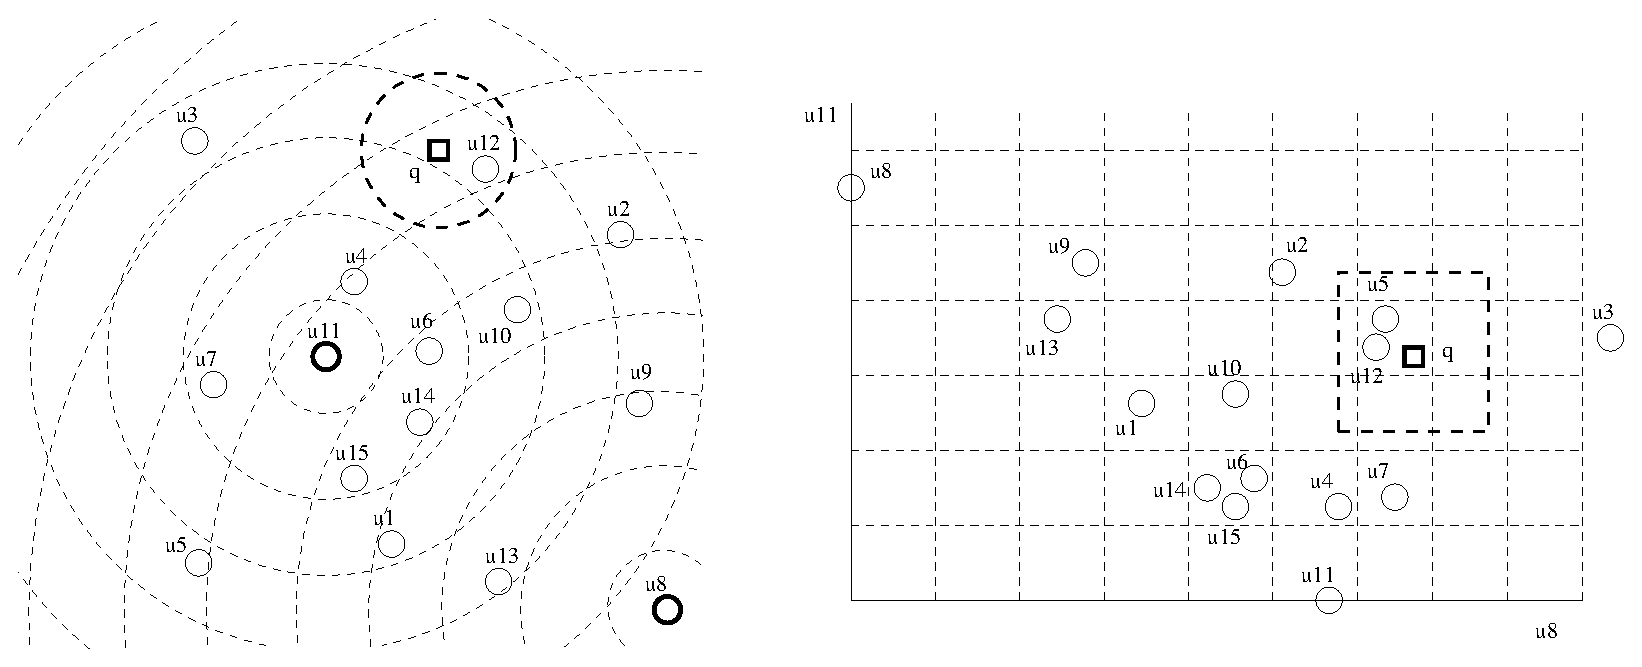
\psfig{file=imagenes/mapeo.eps, width=14cm}}
   \caption [Relaci\'on de equivalencia inducida por dos pivotes y su
   correspondiente transformaci\'on en un espacio vectorial]
     {\textsl{\footnotesize{Sobre la izquierda, un ejemplo de la relaci\'on de equivalencia inducida
        por la intersecci\'on de anillos centrados en dos pivotes, $u_8$ y $u_{11}$.
        Sobre la derecha se ilustra la transformaci\'on en un espacio vectorial de dimensi\'on 2.
    	Tambi\'en se grafica la transformaci\'on de una b\'usqueda $(q,r)_d$. }}}
\label{piv1}
\end{figure}. 

Se puede ver que cada clase de equivalencia est\'a definida por la intersecci\'on de varias capas de esferas centradas en los puntos $p_i$ como se muestra en la figura 2.4.2

Veamos ahora cu\'al ser\'ia una funci\'on de distancia $D$ para las clases de equivalencia.  
Por la desigualdad triangular, para cualquier $x \in X$, se cumple que:

\begin{itemize}
\item 1. $d(p,x) \leq d(p,y) + d(y,x) \Leftrightarrow d(p,x) - d(p,y) \leq d(y,x)$
\item 2. $d(p,y) \leq d(p,x) + d(x,y) \Leftrightarrow d(p,y) - d(p,x) \leq d(x,y)$
\item 3. $d(p,x) - d(p,y) \leq d(y,x) \wedge d(p,y) - d(p,x) \leq d(x,y) \Leftrightarrow |d(x,p) - d(y,p)| \leq d(x,y)$
\end{itemize}

Esto significa que, para cualquier elemento $p$ la distancia $d(x,y)$ no puede ser menor que  
$|d(x,p) - d(y,p)|$. Luego  $D([x],[y]) = |d(x,p) - d(y,p)|$  es un l\'imite inferior seguro 
para $D_0$. Si extendemos $D$ para $k$ los pivotes:

\[
D([x],[y]) = max_{1 \leq i \leq k} \{ |d(x,p_i) - d(y,p_i)|\} 
\]


Esta funci\'on de distancia $D$ limita inferiormente a $d$ y en consecuencia puede usarse como distancia en el espacio cociente.

La relaci\'on de equivalencia definida por un conjunto de $k$ pivotes tambi\'en puede considerarse como una proyecci\'on al espacio vectorial $\Re^k$. La i-\'esima coordenada de un elemento es la distancia al i-\'esimo pivote. Luego, a cada elemento $x$ del espacio le corresponde el vector  $\delta(x) = (d(x,p_1),d(x,p_2),...,d(x,p_k)) \in \Re^k$. Entonces, dada un consulta de b\'usqueda $(q,r)_d$ debemos encontrar un conjunto de elementos candidatos $([q],r)_D = x : D([q],[x]) \leq r$. En este caso particular significa encontrar los elementos tales que:

\[
max_{1 \leq i \leq k} \{ |d(x,p_i) - d(q,p_i)| \} = L_{\infty}(\delta(x),\delta(q)) \leq r 
\]


Esto significa que hemos proyectado el espacio m\'etrico original $(X, d)$ en el espacio
 vectorial $\Re^k$ con la funci\'on de distancia $L_{\infty}$. La Figura \ref{piv1} 
 ilustra estas ideas para un conjunto de puntos usando s\'olo dos pivotes.

\subsection{Algoritmos Basados en Particiones Compactas}


\begin{figure}[tb]
\centerline{%
\begin{minipage}{11cm}
\centerline{ %
   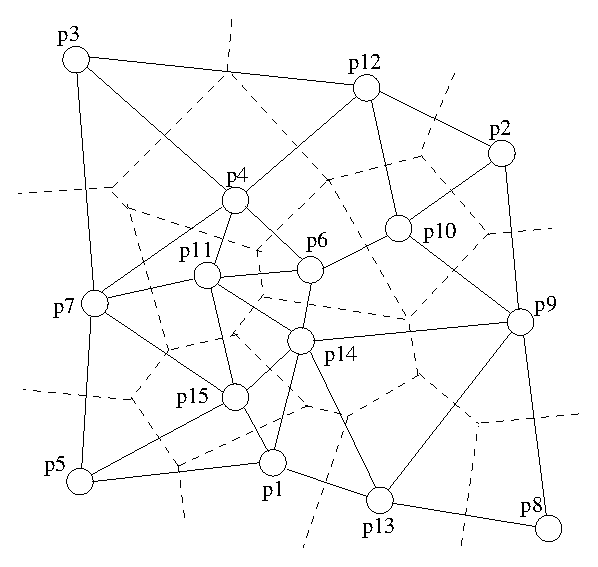
\psfig{file=imagenes/voronoi.eps, width=7cm} }
   \caption [Un ejemplo de Diagrama de Voronoi, y su concepto dual la Triangulaci\'on
      de Delanauy]
   {\textsl{\footnotesize{  Diagrama de Voronoi (l\'ineas punteadas)
     para  un  conjunto de puntos en $\mathbb{R}^2$ con distancia $L_2$; y su concepto
     dual la Triangulaci\'on de Delanauy.}}}
\label{vor-del}
\end{minipage}}
\end{figure}

La idea en este caso es dividir el espacio en particiones o zonas lo m\'as compactas posibles, almacenando puntos representativos de dichas zonas, denominados centros, y algunos datos extra que permitan descartar zonas completas lo m\'as r\'apidamente posible al momento de realizarse una consulta. Cada zona, a su vez, puede ser recursivamente particionada en m\'as zonas, lo cual induce una jerarqu\'ia de b\'usqueda.

\noindent \textbf{\textit{Criterio de partici\'on de Voronoi}}

Los Diagramas de Voronoi \cite{} han sido usados para b\'usquedas por proximidad en espacios vectoriales. Estos diagramas son una de las estructuras fundamentales dentro de la Geometr\'ia Computacional, de alguna forma ellos almacenan toda la informaci\'on referente a la proximidad entre puntos.

Se elige un conjunto de m centros ${c_1,c_2,...,c_m}$. El resto de los objetos se asignan a la zona de su centro m\'as cercano. Cuando todos los objetos de la base de datos son centros, el concepto de partici\'on de Voronoi descrito coincide con el concepto de dominio de Dirichlet [3]. La Figura \ref{vor-del} ejemplifica este concepto en un espacio vectorial 
de dimensi\'on 2.


Al momento de realizar una consulta $(q, r)_d$, se eval\'uan las distancias entre $q$ y los $m$ centros, eligiendo el centro m\'as cercano a $q$, el cual se denominar\'a $c$.

Si la bola de la consulta $(q, r)_d$ intersecta la zona de algun centro distinto a $c$, entonces se debe revisar exhaustivamente esa zona para ver si hay objetos que caigan dentro de la bola de consulta. Sea $x \in X$ un objeto perteneciente a la zona cuyo centro es $c_i$ y que se encuentra a distancia menor o igual que $r$ de la consulta $q$. Por la desigualdad triangular se tiene que:

\begin{enumerate}
\item [1.] $d(c,x) \leq d(c,q) + d(q,x) \leq d(c,q) + r$
\item [2.]$d(c_i,q) \leq d(c_i,x) + d(x,q) \leq d(c_i,x) + r  \Rightarrow d(c_i,q) - r \leq d(c_i,x)$
\end{enumerate}

Como $x$ pertenece a la zona de $c_i$ se cumple que  $d(c_i,x) \leq d(c,x)$. De esta condici\'on m\'as (1) y (2) se obtiene:

\begin{enumerate}
\item [3.] $d(c_i,q) - r \leq d(c_i,x) \leq d(c,x) \leq d(c,q) + r \Rightarrow d(c_i,q) - r \leq d(c,q) + r$
\end{enumerate}

Dada la condici\'on (3), se pueden descartar las zonas cuyo centro $c_i$ satisfaga la condici\'on $d(c_i,q)  > d(c,q) +2r$, dado que en ese caso dicha zona no puede tener intersecci\'on con la bola de consulta

%IMAGEN
%Figura 2.6: Condici\'on de exclusi\'on con criterio de partici\'on de Voronoi.



\section{Dimensi\'on en Espacios M\'etricos}

Uno de los grandes obst\'aculos en el dise\~no de algoritmos de b\'usqueda por similitud es la
llamada maldici\'on de la dimensionalidad \cite{oursurvey}. Si se pudiera representa el conjunto
de elementos de un espacio m\'etrico como puntos en un espacio vectorial, su dimensi\'on 
corresponder\'ia al n\'umero de coordenadas que tienen los puntos que lo componen. 
Todos los algoritmos de b\'usqueda por similitud disminuyen su rendimiento cuando aumenta la  dimensi\'on del conjunto, hecho conocido como maldici\'on de la dimensionalidad. 

En \cite{oursurvey} se muestra que
el concepto de dimensi\'on de un espacio vectorial se puede extender a espacios m\'etricos generales utilizando el concepto de dimensi\'on intr\'inseca, y que la maldici\'on de la dimensionalidad
tiene consecuencias similares en dichos espacios.


La distribuci\'on de distancias de un espacio m\'etrico se define como la probabilidad 
de que dos elementos se encuentre a cierta distancia $l$. Una aproximaci\'on a 
esta distribuci\'on es el \textit{histograma de distancias}, el cual se construye
 desde un subconjunto del espacio m\'etrico, calculando las distancias entre los elementos del subconjunto (ver figura \ref{defineH}).
 
 \begin{figure}[tb!]
\centerline{%
  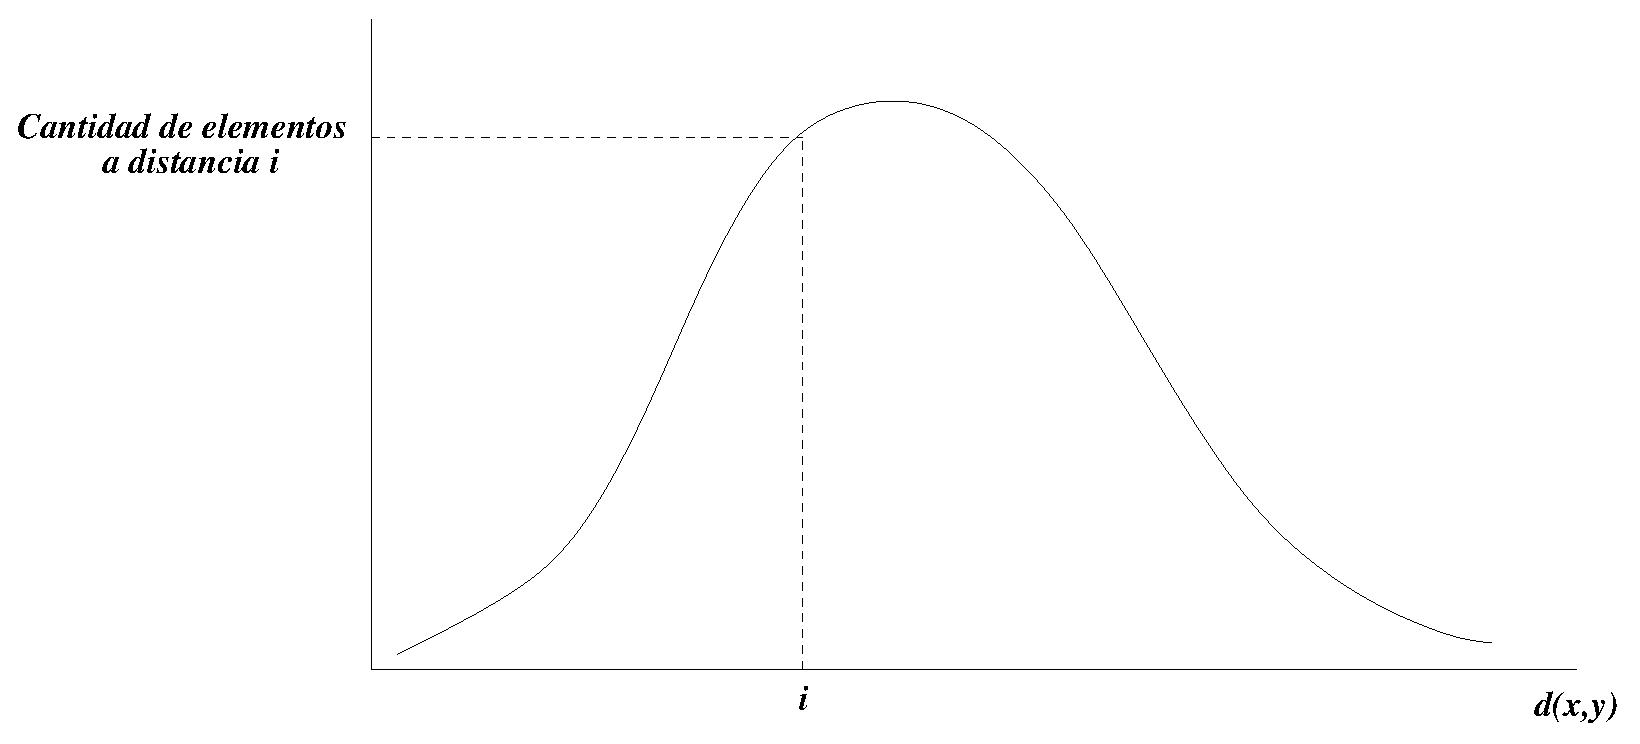
\psfig{file=imagenes/def-histo.eps,width=9cm}}
  \caption [Histograma de distancias de un espacio m\'etrico]
  {\footnotesize {\textsl {Histograma de distancias de un espacio m\'etrico}}}
\label{defineH}
\end{figure}

El histograma de distancias permite visualizar la distribuci\'on de los 
elementos del espacio m\'etrico y se menciona en varios art\'iculos como una medida
 fundamental relacionada a la dimensi\'on intr\'inseca del espacio \cite{Bri95, CM97, cn00,alenex,CPZ98a}. A medida que la dimensi\'on intr\'inseca de un espacio m\'etrico aumenta
la media  $\mu$ del histograma crece y su varianza $\sigma^{2}$ se reduce.

\noindent En \cite{oursurvey} se define la dimensi\'on intr\'inseca de un espacio m\'etrico como:

\[
\gamma = \frac{\mu^2}{2\sigma^2}
\]

Los par\'ametros $\mu$ y $\sigma 2$ son la media y la varianza, respectivamente, del histograma de distancias de los puntos que conforman dicho espacio m\'etrico.



La figura \ref{dim1} da una idea intuitiva de por qu\'e el problema
de b\'usqueda se torna m\'as dif\'icil cuando el histograma es m\'as
concentrado. Consideremos una b\'usqueda $(q,r)_{d}$ y un \'indice
basado en pivotes elegidos aleatoriamente.
En la figura se ejemplifican dos posibles casos para el histograma
local respecto del punto $p$. Si $p$ es un pivote, estas gr\'aficas
representan dos posibles distribuciones para los valores de
$d(q,p)$. La regla de eliminaci\'on dice que podemos descartar aquellos
puntos $y$ tales que  $y \notin [d(p,q)-r, d(p,q) + r]$. Las \'areas sombreadas
muestran  los puntos que no podr\'an descartarse. Esto significa que a medida
que el histograma se concentra m\'as alrededor de su media disminuye la
cantidad de puntos que pueden descartarse usando como dato $d(p,q)$.

Este fen\'omeno es independiente de la naturaleza del espacio
m\'etrico,  y nos brinda una forma de cuantificar cu\'an dif\'icil es una
b\'usqueda sobre el mismo. Tal como se muestra experimental y anal\'iticamente
en \cite{oursurvey}, todos los algoritmos degradan  sistem\'aticamente
cuando la media $\rho$ del espacio se incrementa.

\begin{figure}[tb]
\centerline{%
  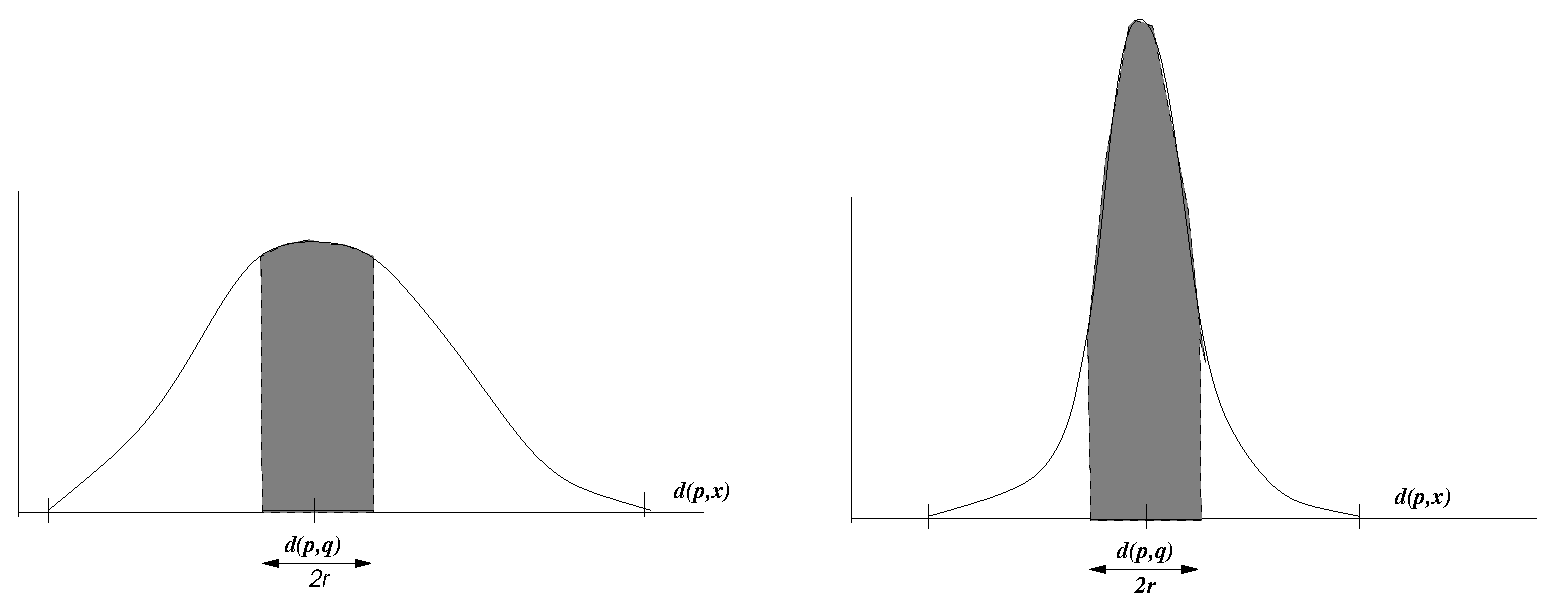
\psfig{file=imagenes/histog.eps,width=14cm}}
  \caption [Histogramas de distancias de baja y
             alta dimensionalidad]
    { \textsl{\footnotesize Histogramas de distancias de baja dimensionalidad
                (izquierda), y  de alta dimensionalidad (derecha)}}
\label{dim1}
\end{figure}

%\subsection{La maldici\'on de la dimensionalidad}
%
%Cuando se realiza una consulta por rango, los algoritmos basados en pivotes intentan descartar la mayor cantidad de elementos del espacio m\'etrico antes de realizar una b\'usqueda exhaustiva. Esto es, se genera una lista de elementos candidatos en la cual se verifica exhaustivamente la condici\'on de b\'usqueda.
%
%Si nos centramos nuevamente en el histograma de distancias de un espacio m\'etrico $(E, d)$, es f\'acil ver que seg\'un la condici\'on de exclusi\'on de elementos (ECUACION), dada una consulta $(q, r)$ y un conjunto de $k$ pivotes $p_i$, se pueden descartar todos los elementos $x \in E$ que no cumplan para alg\'un $i \in 1..k$ la condici\'on de la siguiente ecuaci\'on:
%
%\[
%d(p_i, x) \notin [d(p_i, q) - r , d(p_i, q) + r]
%\]
%
%Mientras m\'as grande es la dimensi\'on intr\'inseca del espacio m\'etrico, la media del histograma aumenta y/o disminuye la varianza.
%
%Cuando la varianza del histograma disminuye a medida que aumenta la dimensi\'on del espacio,
% el n\'umero de elementos que se encuentran dentro del rango $[d(p, q)-r , d(p, q)+r ]$ tambi\'en 
% aumenta, es decir que cada vez son menos los elementos que se pueden descartar. Alternativamente, 
% si la media crece entonces $r$ tambi\'en crece con la dimensi\'on del espacio si se quiere 
% obtener un porcentaje fijo de elementos del conjunto. En espacios de alta dimensionalidad, casi 
% todos los elementos se transforman en candidatos a la verificaci\'on exhaustiva, por lo que deben 
% ser comparados directamente con la consulta. A esto se le denomina \textit{maldici\'on de la 
% dimensionalidad}, y es independiente de la naturaleza del espacio m\'etrico al cual pertenecen 
% los elementos.


%PARA CAP 3
%\section{T\'ecnicas de Selecci\'on de Pivotes}
%En este trabajo nos hemos centrado en algoritmos basados en pivotes, por lo que
%analizaremos el tema de c\'omo seleccionar los pivotes al momento de indexar el espacio 
%m\'estrico.
%
%La forma en que los pivotes son seleccionados puede afectar dr\'asticamente la performance de un 
%algoritmo. Una buena elecci\'on de pivotes puede en gran parte reducir los tiempos de b\'usqueda.
%
%\subsection{Criterios de eficiencia}
%
%Es necesario minimizar el n\'umero de evaluaciones de distancia que se realizan al momento de 
%hacer una b\'usqueda por rango. Para lograr esto, los pivotes elegidos deben descartar la mayor 
%cantidad de los elementos posibles antes de realizar una b\'usqueda dentro de una lista de 
%elementos candidatos. En s\'intesis, un buen conjunto de pivotes debe generar una lista peque\~na 
%de elementos candidatos.
%
%Sea $(X,d)$ un espacio m\'etrico. Un conjunto de pivotes $\{p_1,p_2,...,p_k\} \in X$ definen un 
%espacio $P$ de tuplas de distancias entre pivotes y elementos del conjunto. Un elemento $x \in P$ 
%se denotar\'a como $[x]$ que es igual a la siguiente ecuaci\'on:
%
%\begin{equation}
%[x] = (d(x,p_1),d(x,p_2),........,d(x,p_k)), x \in X, [x] \in P
%\end{equation}
%
%
%\noindent Definimos la m\'etrica $D = D_{\{p_1,...,p_k\}}$ del espacio $P$ como:
%
%\begin{equation}
%D([q],[x]) = max_{i=1}^k |d(q,p_i) - d(x,p_i)|
%\end{equation}
%
%Luego, obtenemos el espacio m\'etrico $(X,D)$ que resulta ser $(\Re^k, L_{\infty})$. Dada una consulta por rango $(q,r)$ es f\'acil ver este nuevo espacio m\'etrico, que seg\'un la condici\'on de la ecuaci\'on 2-6, no se pueden excluir aquellos elementos  $x \in E$ que cumplen con:
%
%\begin{equation}
%D_{\{p_1,...,p_k\}}([q],[x]) \leq r
%\end{equation}
%
%Para lograr que la cantidad de elementos elegidos sea peque\~na se debe maximizar la probabilidad de que $D_{\{p_1,...,p_k\}}([q],[x]) > r$. Una forma de lograr esto es maximizar la media de la distribuci\'on de distancias en $P$, la cual la llamaremos $\mu_p$.
% 
%\subsection{Estimaci\'on del $\mu_p$}
%
%\noindent La estimaci\'on del $\mu_p$ se realiza de ls siguiente manera:
%
%\begin{itemize}
%
%\item Elegir $A$ pares de elementos $\{(a_1,a'_1),(a_2,a'_2),.......,(a_A,a'_A)\}$ 
%del conjunto $E$, distintos entre s\'i.
%
%\item Mapear los $A$ pares de elementos al espacio $P$ y calcular la distancia $D$ entre
% cada par de elementos, esto produce como resultado el conjunto finito de distancias
%  $\{D_1,D_2,...,D_A\}$.
%  
%\item Luego de obtener las $A$ distancias se estima el valor de $p$ de la siguiente forma:
%\end{itemize}
%
%\begin{equation}
%\mu_p = \frac{\sum_{i=1}^A D_i}{A}
%\end{equation}
%
%De las ecuaciones 2.5.1 y 2.5.2, se puede deducir que dados un  par de elementos $(a,a')$ 
%el costo de calcular $D([a],[a'])$ es $2k$ evaluaciones de la funci\'on $d$.
%
%Se se utilizan $A$ pares de elementos para estimar el valor de $\mu_p$ , se puede ver
% que el costo total de la estimaci\'on es de $2kA$ evaluaciones de la funci\'on $d$.
%
%\subsection{M\'etodos de selecci\'on de pivotes}
%
%En este trabajo vamos a describir los dos m\'etodos de selecci\'on utilizados y sus costos en funci\'on al n\'umero de evaluaciones de la distancia $d$.
%
%\noindent \textit{\textbf{Selecci\'on Random}}
%
%Esta t\'ecnica consiste en la elecci\'on al azar de los pivotes, no se usa ning\'un criterio de selecci\'on. 
%\
%En este trabajo mostraremos la diferencia o beneficios en las b\'usquedas al usar pivotes seleccionados usando t\'ecnicas incrementales versus la selecci\'on aleatoria de pivotes.
%\
%El costo de optimizar los pivotes usando selecci\'on random es $0$
%
%\noindent \textit{\textbf{Selecci\'on Incremental}}
%
%El m\'etodo consiste en elegir un pivote $p_1$ utilizando $A$ pares de elementos del espacio $E$ mapeados a $P$, tal que \'ese pivote maximice el $\mu_p$. Luego elegir un segundo pivote $p_2$, tal que $\{p_1,p_2\}$ maximicen $\mu_p$ pero $p_1$ ya queda fijo. Luego elegir un tercer pivote $p_3$, tal que $\{p_1,p_2,p_3\}$  maximicen $\mu_p$ pero con $p_1$ y  $p_2$ fijos. Repetir el proceso hasta elegir los $k$ pivotes.
%
%En cada iteraci\'on se elige un pivote de una muestra de tama\~no $X$ del espacio $E$, 
%dado que buscar un elemento que maximice $\mu_p$ dentro del todo el conjunto 
%$E$  ser\'ia muy costoso.
%
%\noindent \textit{Costo del algoritmo}:
%
%Si bien en cada iteraci\'on se estima el $\mu_p$ con los $i$ pivotes seleccionados hasta el 
%momento, no es necesario rehacer el c\'alculo completo si se almacena $D_{\{p_1,...,p_{i-1}\}}
%([a_r],[a'_r]) \forall r \in 1..A$, es decir, para cada valor de $r=1..A$ el valor m\'aximo de $|
%d(a'_r, p_j) - d(a_r, p_j)|, j = 1..i-1$. En este caso solo se calcula la distancia con respecto a 
%los pivotes candidatos $|d(a'_r, p_{cand}) - d(a_r, p_{cand})|, r = 1..A$ y se toma el valor m
%\'aximo entre las dos distancias para el calculo de $D\{p_1, ...,p_i\}$. Entonces, si la muestra 
%de donde se toman los pivotes candidatos es de tama\~no $X$, en cada iteraci\'on se realizan $2AX$ 
%evaluaciones de la funci\'on $d$. Luego, si se eligen $k$ pivotes, el trabajo total realizado por 
%el algoritmo tiene un costo de $2kAX$ evaluaciones de la funci\'on $d$.
%
%
%

%\section{B\'usquedas por Similitud}
%
%Como ya mencionamos anteriormente, en este trabajo nos interesa realizar b\'usquedas por similitud; esto es, dada una consulta $q$, queremos encontrar todos aquellos objetos del universo de inter\'es que est\'an cercanos a $q$, bajo una funci\'on de distancia dada. B\'asicamente, existen tres tipos de b\'usquedas por similitud:
%
%\begin{enumerate}
%\item [1.] B\'usquedas por rango.
%\item [2.] B\'usquedas del vecino m\'as cercano. 
%\item [3.] B\'usquedas de los $k$ vecinos m\'as cercanos.
%\end{enumerate}
%
%Explicamos a continuaci\'on cada una de ellas.
%
%\subsection{B\'usquedas por rango}
%
%Las b\'usquedas por rango $R(q,r)$ son probablemente las m\'as comunes dentro de los espacios
% m\'etricos. En estas b\'usquedas, la consulta se define como un objeto $q \in D$, especificando 
% un radio $r$ como una restricci\'on de distancia. Dicha b\'usqueda devuelve todos los objetos 
% encontrados a una distancia $r$ de $q$, formalmente:
%
%
%\begin{equation}
%R(q,r) = {o \in X, d(o,q) \leq r}
%\end{equation}
%
%Los objetos pertenecientes a la respuesta pueden ordenarse en base a su distancia de $q$, si es necesario. N\'otese que el objeto $q$ no necesita existir en el conjunto $X \subseteq D$ en el cual se busca, y la \'unica restricci\'on sobre q es que pertenezca al dominio D.
%
%En la figura 1.2a se muestra un ejemplo de b\'usqueda por rango.
%
%\subsection{B\'usquedas del vecino m\'as cercano}
%
%Cuando se quiere realizar b\'usquedas por similitud sobre objetos utilizando b\'usquedas por rango, se debe especificar la distancia m\'axima para que los objetos sean inclu\'idos en la respuesta; pero en ocasiones puede ser dif\'icil especificar el radio sin conocimiento sobre los datos y la funci\'on de distancia. Por ejemplo, $r=3$ de la m\'etrica de distancia de edici\'on representa menos de cuatro operaciones de edici\'on entre dos cadenas comparadas; \'esto tiene un claro significado sem\'antico. Sin embargo, una distancia entre dos vectores de histograma de colores de im\'agenes es un n\'umero real cuya cuantificaci\'on no puede ser interpretada tan f\'acilmente.
%
%Existe entonces, la situaci\'on en donde, si especificamos un radio de b\'usqueda muy peque\~no no obtendremos ning\'un resultado, y deberemos repetir la b\'usqueda con un radio mayor. Por otro lado, si especificamos un radio de b\'usqueda muy grande, corremos el riesgo de que el costo computacional de calcular la distancia sea muy alto y de que el conjunto de resultados contenga objetos no significativos.
%
%Una alternativa para solucionar este tipo de problemas en la b\'usqueda por similitud es realizar una b\'usqueda de los vecinos m\'as cercanos. B\'asicamente dicha b\'usqueda consiste en encontrar el objeto m\'as cercano a la consulta $q$, al que denominamos vecino m\'as cercano de $q$.
%
%\subsection{B\'usquedas de los k vecinos m\'as cercanos}
%
%El concepto de vecino m\'as cercano puede generalizarse al caso de b\'usqueda de los $k$ vecinos m\'as cercanos. Espec\'ificamente $kNN(q)$ retorna los $k$ vecinos m\'as cercanos del objeto $q$, y dicho conjunto resultado se define formalmente como:
%
%\begin{equation}
%kNN(q)={ R \subseteq X, |R|=k \wedge \forall x \in R, y \in X-R : d(q,x) \leq d(q,y)}
%\end{equation}
%
%
%Cuando existen varios objetos a la misma distancia del $k$-\'esimo vecino m\'as cercano, la elecci\'on de uno se realiza arbitrariamente. La figura 2.2b ilustra la situaci\'on para una consulta $3NN(q)$; en ella los objetos $o_1,o_3$ est\'an ambos a distancia $3.3$ y el objeto $o_1$ es elegido como tercer vecino m\'as cercano en forma aleatoria en vez de $o_3$.
%
%IMAGEN
%
%Figura 2.2: (a) B\'usqueda por rango R(q,r) y (b) b\'usqueda del vecino m\'as cercano 3NN(q).
%
